\documentclass[letterpaper]{article}
\usepackage[margin=1in]{geometry}
\usepackage[utf8]{inputenc}
\usepackage{textcomp}
\usepackage{amssymb}
\usepackage{natbib}
\usepackage{graphicx}
\usepackage{gensymb}
\usepackage{amsthm, amsmath, mathtools}
\usepackage[dvipsnames]{xcolor}
\usepackage{enumerate}
\usepackage{mdframed}
\usepackage[most]{tcolorbox}
\usepackage{csquotes}
% https://tex.stackexchange.com/questions/13506/how-to-continue-the-framed-text-box-on-multiple-pages

\tcbuselibrary{theorems}

\newcommand{\R}{\mathbb{R}}
\newcommand{\Z}{\mathbb{Z}}
\newcommand{\N}{\mathbb{N}}
\newcommand{\Q}{\mathbb{Q}}
\newcommand{\C}{\mathbb{C}}
\newcommand{\code}[1]{\texttt{#1}}
\newcommand{\mdiamond}{$\diamondsuit$}
\newcommand{\PowerSet}{\mathcal{P}}
\newcommand{\Mod}[1]{\ (\mathrm{mod}\ #1)}
\DeclareMathOperator{\lcm}{lcm}

%\newtheorem*{theorem}{Theorem}
%\newtheorem*{definition}{Definition}
%\newtheorem*{corollary}{Corollary}
%\newtheorem*{lemma}{Lemma}
\newtheorem*{proposition}{Proposition}


\newtcbtheorem[number within=section]{theorem}{Theorem}
{colback=green!5,colframe=green!35!black,fonttitle=\bfseries}{th}

\newtcbtheorem[number within=section]{definition}{Definition}
{colback=blue!5,colframe=blue!35!black,fonttitle=\bfseries}{def}

\newtcbtheorem[number within=section]{corollary}{Corollary}
{colback=yellow!5,colframe=yellow!35!black,fonttitle=\bfseries}{cor}

\newtcbtheorem[number within=section]{lemma}{Lemma}
{colback=red!5,colframe=red!35!black,fonttitle=\bfseries}{lem}

\newtcbtheorem[number within=section]{example}{Example}
{colback=white!5,colframe=white!35!black,fonttitle=\bfseries}{def}

\newtcbtheorem[number within=section]{note}{Important Note}{
        enhanced,
        sharp corners,
        attach boxed title to top left={
            xshift=-1mm,
            yshift=-5mm,
            yshifttext=-1mm
        },
        top=1.5em,
        colback=white,
        colframe=black,
        fonttitle=\bfseries,
        boxed title style={
            sharp corners,
            size=small,
            colback=red!75!black,
            colframe=red!75!black,
        } 
    }{impnote}
\usepackage[utf8]{inputenc}
\usepackage[english]{babel}
\usepackage{fancyhdr}
\usepackage[hidelinks]{hyperref}

\pagestyle{fancy}
\fancyhf{}
\rhead{Math 103B}
\chead{Wednesday, January 05, 2022}
\lhead{Lecture 2}
\rfoot{\thepage}

\setlength{\parindent}{0pt}

\begin{document}

\section{Properties of Rings}
We begin by talking about a few important properties. 

\subsection{Basic Rules of Multiplication}
\begin{theorem}{}{}
    For all $a \in R$, we have: 
    \[a0 = 0a = 0\]
\end{theorem}

\begin{mdframed}[]
    \begin{proof}
        We know that: 
        \[0a = (0 + 0)a = 0a + 0a\]
        Subtracting both sides by $0a$ gives: 
        \[0 = 0a + (0a - 0a) \implies 0 = 0a\]
        By symmetry, we can do the same for $0a$. Therefore, we are done.
    \end{proof}    
\end{mdframed}

\begin{theorem}{}{}
    For all $a, b \in R$, we have:
    \[a(-b) = (-a)b = -(ab)\]
\end{theorem}

\begin{mdframed}[]
    \begin{proof}
        First, we have: 
        \[a(-b) + ab = a(-b + b) = a0 = 0\]
        Now, if we add $-(ab)$ to both sides, we have: 
        \[a(-b) + ab + -(ab) = -(ab) \implies a(-b) = -(ab)\]
        By symmetry, $(-a)b = -(ab)$ as well. 
    \end{proof}
\end{mdframed}

\begin{theorem}{}{}
    For all $a, b \in R$, we have: 
    \[(-a)(-b) = ab\]
\end{theorem}

\begin{mdframed}[]
    \begin{proof}
        \begin{equation*}
            \begin{aligned}
                (-a)0 &= 0 \\ 
                    &\iff (-a)(b + (-b)) = 0 \\ 
                    &\iff (-a)b + -a(-b) = 0 \\ 
                    &\iff -(ab) + -a(-b) = 0 \\ 
                    &\iff ab + -(ab) + -a(-b) = ab \\
                    &\iff -a(-b) = ab
            \end{aligned}
        \end{equation*}
        So, we are done. 
    \end{proof}
\end{mdframed}

\begin{theorem}{}{}
    For all $a, b, c \in R$, we have: 
    \[a(b - c) = ab - ac \text{ and } (b - c)a = ba - ca\]
\end{theorem}

\begin{mdframed}[]
    \begin{proof}
        \begin{equation*}
            \begin{aligned}
                a(b - c) &= ab + -(ac) \\ 
                    &= ab + (-a)c \\ 
                    &= ab - ac
            \end{aligned}
        \end{equation*}
        By symmetry, we can apply the other side as well. So, we are done. 
    \end{proof}
\end{mdframed}

\subsection{Rules of Multiplication with Unity Element}
\begin{theorem}{}{}
    For all $a \in R$ where $R$ has a unity element 1, we have: 
    \[(-1)a = -a\]
\end{theorem}

\begin{mdframed}[]
    \begin{proof}
        Applying the theorem that we proved:
        \[(-1)a = -(1a) = -a\]
        So, we are done. 
    \end{proof}
\end{mdframed}

Alternatively:
\begin{mdframed}[]
    \begin{proof}
        Since $(\R, +)$ is an abelian group, it suffices to prove that $(-1)a + a = 0$.
        \[(-1)a + a = (-1)a + 1a = (-1 + 1)a = 0a = 0\]
        So, we are done. 
    \end{proof}
\end{mdframed}

\begin{theorem}{}{}
    \[(-1)(-1) = 1\]
\end{theorem}

\begin{mdframed}[]
    \begin{proof}
        Applying the theorem that we proved:
        \[(-1)(-1) = 1(1) = 1\]
        So, we are done.
    \end{proof}
\end{mdframed}

\subsection{Uniqueness of Unity and Inverses}
\begin{theorem}{}{}
    If a ring has a unity, it is unique. If a ring element has a multiplicative inverse, it is also unique. 
\end{theorem}

\begin{mdframed}[]
    \begin{proof}
        We will prove both parts individually. Suppose $R$ is a ring.  
        \begin{enumerate}
            \item Suppose $e$ and $e'$ are unity elements in a ring $R$. Then, we know that: 
            \begin{itemize}
                \item $e = ee'$ since $e'$ is a unity. 
                \item $e' = ee'$ since $e$ is a unity. 
            \end{itemize}
            Therefore: 
            \[e = ee' = e'\]
            Which means that the unity must be unique. 

            \item Suppose $a \in R$ and further suppose that $x$ and $y$ are both multiplicative inverses of $a$. Then: 
            \[x = x1 = x(ay) = (xa)y = 1y = y\]
            Therefore, $x = y$ and the two inverses are equal. 
        \end{enumerate}
        Therefore, we are done. 
    \end{proof}
\end{mdframed}

\begin{note}{}{}
    Rings are not groups under multiplication. $R - \{0\}$ is not a group under multiplication. \underline{Rings may not have multiplicative cancellations.}
\end{note}
To show that this is the case, consider the question: Which elements $a \in R$ satisfy $a^2 = a$?
\begin{itemize}
    \item If $R$ has unity, then $a = 1$.
    \item $a = 0$ is always a solution.
\end{itemize}
Now, consider $\Z / 6 \Z = \{0, 1, 2, 3, 4, 5\}$. Then, $a^2 = a$ for $a = 0, 1, 3, 4$. The only units in this ring are 1 and 5. 


\newpage 
\section{Subring}
Recall that, with groups, we have objects called \emph{subgroups}. The same thing applies here: with rings, we have objects called \emph{subrings}.
\begin{definition}{Subring}{}
    A nonempty subset $S$ of a ring $R$ is a \textbf{subring} of $R$ if $S$ itself is a ring with the operations of $R$.
\end{definition}

\subsection{Examples of Subrings}
Below are some examples of subrings. 

\subsubsection{Example 1: Simple Subrings}
The trivial subring $\{0\}$ is a subring of any ring $R$. This is because:
\[0(0) \in R \qquad 0 - 0 \in R\]
Any ring $R$ is a subring of itself. This is because for any $a, b \in R$, we know that $a - b = a + (-b) \in R$ and $ab \in R$. 

\subsubsection{Example 2: Integers}
For any positive integer $n$, the set below is a subring of the integers $\Z$: 
\[n\Z = \{0, \pm n, \pm 2n, \pm 3n, \dots\}\]
Take any $a, b \in \Z$. Then, suppose we have $an$ and $bn$. We know that: 
\[an - bn = (a - b)n \in \Z\]
\[an(bn) = anbn\]
Since $anb \in \Z$, it follows that $(anb)n \in n\Z$. 

\subsubsection{Example 3: Rational Numbers}
The ring $\Q$ is a subring of $\R$. 


\subsubsection{Example 4: Gaussian Integers}
Consider the Gaussian integers:
\[\Z[i] = \{a + bi \mid a, b \in \Z\}\]
This is a subring of $\C$. Note that $i^2 = -1$ so:
\[(a + bi)(c + di) = ac + adi + bci + bdi^2 = ac + adi + bci - bd = (ac - bd) + (ad + bc)i\]

\subsubsection{Example 5: Integers with Square Root 2}
Consider the following set: 
\[\Q[\sqrt{2}] = \{a + b\sqrt{2} \mid a, b \in \Q\}\]
This is a subring of $\R$. This is because: 
\[(a + b\sqrt{2})(c + d\sqrt{2}) = ac + ad\sqrt{2} + bc\sqrt{2} + 2bd\]
Note that we can apply the same work used in the previous example. 

\subsubsection{Example 7: Diagonal Matrices}
The set of diagonal matrices is a subring of $M_{2}(\Z)$. 
\[\left\{\begin{bmatrix}
    a & 0 \\ 0 & d
\end{bmatrix} \mid a, d \in \Z\right\}\]


\subsection{Subring Test}
\begin{theorem}{Subring Test}{}
    A nonempty subset $S$ of a ring $R$ is a subring if $S$ is closed under subtraction and multiplication; that is, if $a - b \in S$ and $ab \in S$ whenever $a, b \in S$. 
\end{theorem}

\begin{mdframed}[]
    \begin{proof}
        If $S$ is a subring, then it is a ring and so $S$ must be closed under subtraction and multiplication. 

        \bigskip 

        Suppose $S$ is closed under subtraction and multiplication. Then, we know the following properties (inherited from $R$): 
        \begin{itemize}
            \item $a + b = b + a$
            \item $(a + b) + c = a + (b + c)$
            \item $a(bc) = (ab)c$
            \item $a(b + c) = ab + ac$
            \item $(a + b)c = ac + bc$
        \end{itemize}
        We need to check if $S$ has 0. Since $S$ is not empty, pick some $a \in S$. Then, it follows that: 
        \[a - a = 0 \in S\]
        So, the additive identity exists. Now, if $a \in S$, then $-a = 0 - a \in S$, so additive inverses exist. 

        \bigskip 

        Finally, we need to show that addition is closed. We know that subtraction is closed, so if $a, b \in S$, then $-b \in S$ and $a + b = a - (-b) \in S$. 
    \end{proof}
\end{mdframed}

\subsection{Subring Lattice}
If we are dealing with a lot of subrings, we can use a \emph{subring lattice} to better show the relationship between these rings. An example of a subring lattice is: 
\begin{center}
    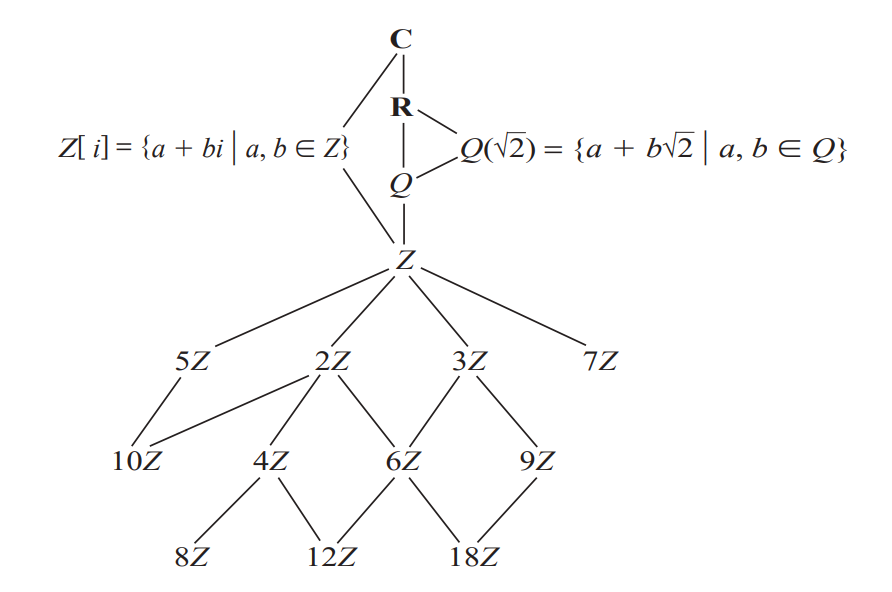
\includegraphics[scale=0.5]{../assets/lattice.png}
\end{center}
We used some of the examples discussed above.

\end{document}